\section{Definition of Minimal Obstructions} \label{sec:definition_of_obstructions}

In this section, we formally define all twelve classes of minimal obstructions which make a partial
representation non-extendible. 

\heading{Definition.}
Every \emph{obstruction} consists of a graph $H$ and a non-extendible partial representation $\calR'_H$.
This obstruction is \emph{contained} in $G$ and $\calR'$ if (i) $H$
is an induced subgraph of $G$, (ii)~the pre-drawn vertices of $H$ are mapped to pre-drawn vertices of
$G$, and (iii) the endpoints in $\calR'_H$ have the same left-to-right order as the endpoints of the
corresponding pre-drawn vertices in $\calR'$. For instance, the partial representation in
Fig.~\ref{fig:int_example}b contains a $1$-FAT obstruction, given in Fig.~\ref{fig:minimal_obstructions}a.

We give $H$ by \emph{descriptions} using finitely many vertices, edges, and induced paths. For inner
vertices of the induced paths, we specify their adjacencies with the remainder of $H$. Since these
induced paths do not have fixed lengths, each description having at least one induced path defines
an infinite class of forbidden subgraphs $H$. Unlike LB obstructions, most classes of minimal
obstructions need infinitely many different descriptions. For instance, each FAT obstruction has $k$
induced paths, and different values of $k$ need different descriptions.

If $H$ contains an induced path $P_{x,y}$, and $x$ and $y$ are allowed to be adjacent, then
$P_{x,y}$ can be a single edge.  When $N[x] = N[y]$, we allow the length of $P_{x,y}$ to be zero,
i.e., $x=y$.

\heading{Minimality.} An obstruction is \emph{minimal} if $\calR'_H$ becomes extendible when any
vertex is removed or any pre-drawn interval is made \emph{free} by removing it from the partial
representation $\calR'_H$. 

\subsection{List of Minimal Obstructions}

In Fig.~\ref{fig:LB_obstructions}, we have already described minimal LB obstructions
of~\cite{lb_graphs} with $\calR'_H = \emptyset$.  There are eleven other other classes of minimal
obstructions we describe now. 

\begin{figure}[t!]
\centering
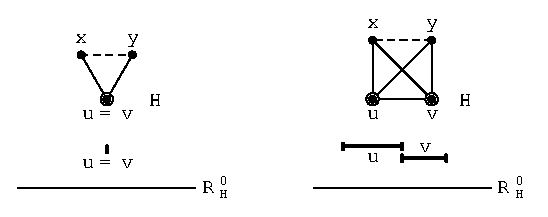
\includegraphics{definition_of_obstructions_SE.eps}
\caption{The SE obstructions, on the left with $u=v$, on the right with $u \ne v$.}
\label{fig:SE}
\end{figure}

\begin{figure}[b!]
\centering
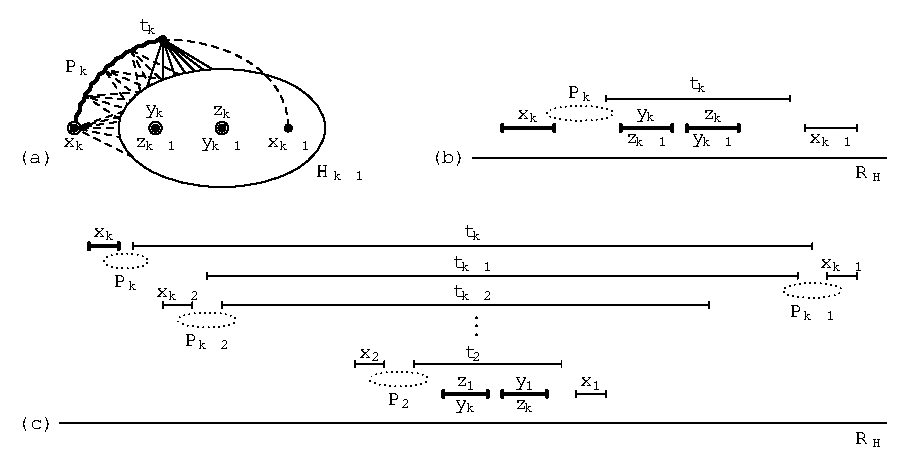
\includegraphics{definition_of_obstructions_k_FAT.eps}
\caption[ ]{(a) A $k$-FAT obstruction is created from a $(k-1)$-FAT obstruction. It consists of the
vertices $x_1,\dots,x_k$, $t_2,\dots,t_k$, $y_k$, $z_k$, and the induced paths $P_1,\dots,P_k$. The
adjacencies are defined inductively.\\
(b) In every representation $\calR_H$, the pre-drawn interval $\inter{x_k}'$ together with $P_k$ and
$t_k$ forces $\inter{x_{k-1}}$ to be placed on the right of $\inter{z_k}'$. Therefore, the induced
$(k-1)$-FAT obstruction is forced.\\
(c) The global zig-zag pattern forced by a $k$-FAT obstruction, with $k$ nested levels going across
$\inter{y_k}'$ and $\inter{z_k}'$. It is an obstruction since $P_1$ going from $x_1$ to $z_1$ with
all inner vertices non-adjacent to $y_1$ cannot be placed.}
\label{fig:k_FAT}
\end{figure}

\heading{SE obstructions.} We start with two simple \emph{shared endpoint obstructions} which deal
with shared endpoints in $\calR'$; see Fig.~\ref{fig:SE}. We have two pre-drawn vertices $u$ and
$v$ such that $r(u) = \ell(v)$ (possibly $u=v$, so only one interval may be pre-drawn). Further,
there are two non-adjacent vertices $x$ and $y$, both adjacent to $u$ and $v$.  If $u \ne v$, the
minimality requires that $\ell(u) < \ell(v) = r(u) < r(v)$.

\heading{$\boldsymbol{k}$-FAT obstructions.} The class of \emph{forced asteroidal triple obstructions}
is defined inductively; the first two obstructions $1$-FAT and $2$-FAT are depicted in
Fig.~\ref{fig:minimal_obstructions}a and b, respectively.

A $1$-FAT obstruction consists of three pre-drawn non-adjacent vertices $x_1$, $y_1$ and $z_1$ such
that $\inter{y_1}'$ is between $\inter{x_1}'$ and $\inter{z_1}'$. Further, $x_1$ and $z_1$ are
connected by an induced path $P_1$ and $y_1$ is non-adjacent to the inner vertices of $P_1$. See
Fig.~\ref{fig:minimal_obstructions}a.

A $k$-FAT obstruction is defined as follows; see Fig.~\ref{fig:k_FAT}a.  Let $H_{k-1}$ be the graph
of a $(k-1)$-FAT obstruction.  To get $H_k$, we add to $H_{k-1}$ two vertices $x_k$ and $t_k$
connected by an induced path $P_k$.   Concerning edges, $t_k$ is adjacent to all vertices of
$H_{k-1}$, except for $x_{k-1}$. All vertices of $H_{k-1}$ are non-adjacent to $x_k$ and to the
inner vertices of $P_k$.  Further, for $k > 1$, we allow $P_1$ to be a single edge, so $x_1$
can be adjacent to $z_1$.

We put $y_k = z_{k-1}$ and $z_k = y_{k-1}$.  A $k$-FAT obstruction has three pre-drawn vertices
$x_k$, $y_k$ and $z_k$ such that $\inter{y_k}'$ is between $\inter{x_k}'$ and $\inter{z_k}'$.  The
role of $\inter{x_k}'$, $P_k$ and $t_k$ is to force $\inter{x_{k-1}}$ to be placed on the other side of
$\inter{z_k}' = \inter{y_{k-1}}'$ than $\inter{y_k}' = \inter{z_{k-1}}'$, thus forcing the
$(k-1)$-FAT obstruction of $H_{k-1}$; see Fig.~\ref{fig:k_FAT}b. The global structure forced by a
$k$-FAT obstruction is depicted in Fig.~\ref{fig:k_FAT}c. 

\begin{figure}[b!]
\centering
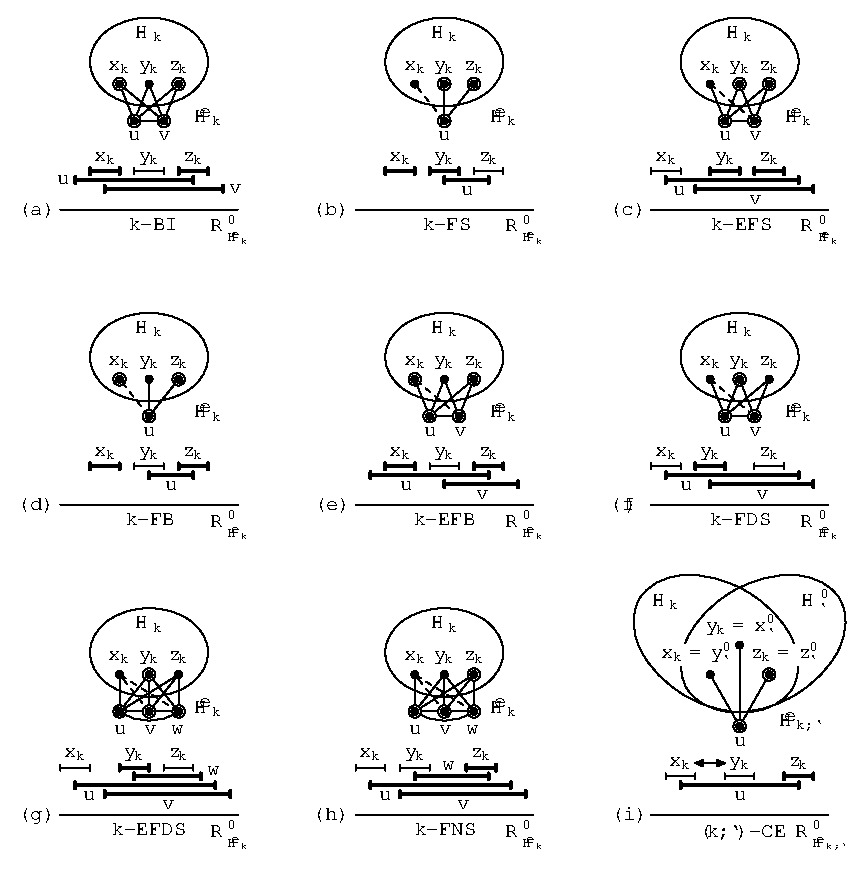
\includegraphics{definition_of_obstructions_overview_of_obstructions.eps}
\caption[ ]{Nine classes of obstructions derived from $k$-FAT obstructions.}
\label{fig:overview_of_obstructions}
\end{figure}

The remaining nine classes, depicted in Fig.~\ref{fig:overview_of_obstructions}, are derived from
$k$-FAT obstructions. Let $H_k$ denote the graph of a $k$-FAT obstruction. With exception of the
last class of $(k,\ell)$-CE obstructions, we create the graphs $\widetilde H_k$ of these
obstructions by adding a few vertices to $H_k$. For $k=1$, when one of $x_1$ and $z_1$ is not
pre-drawn, we also allow $x_1$ to be adjacent to $z_1$. We also consider all of these
obstructions horizontally flipped.

It is possible that the added vertices already belong to $H_k$; for instance, a $k$-BI obstruction
may have $u = t_k$ or $v = t_k$.  Also, we do not specify in details the edges between the added
vertices and $H_k \setminus \{x_k, y_k, z_k\}$.  An accurate description would be too lengthy and
the reader may derive it from Fig.~\ref{fig:k_FAT}c.  We describe all minimal $(k,\ell)$-CE
obstructions in details.

\heading{$\boldsymbol{k}$-BI obstructions.} The class of \emph{blocked intersection
obstructions} is shown in Fig.~\ref{fig:overview_of_obstructions}a. To create $\widetilde H_k$ from $H_k$, we add
two vertices $u$ and $v$ adjacent to $x_k$, $y_k$ and $z_k$. Then the partial
representation contains four pre-drawn vertices $x_k$, $z_k$, $u$ and $v$.
We have $\ell(u) \le \ell(v) < r(u) \le r(v)$, $\inter{x_k}'$ covering $\ell(v)$, and
$\inter{z_k}'$ covering $r(u)$. We allow $u = v$. 

The minimality further implies that $k \le 2$. Indeed, a $k$-BI obstruction with $k>3$ contains a smaller
$(k,1)$-CE obstruction by removing $v$ and freeing $\inter{x_k}'$ (this follows from
Lemma~\ref{lem:k_fat_contains_1_fat}). Concerning $1$-BI, we allow $x_1 = z_1$. We illustrate all possible cases only for $1$-BI
obstructions, so the reader can understand the complexity of these classes; see
Fig.~\ref{fig:BI_obstructions}.  For $k=2$, we know by Lemma~\ref{lem:k_fat_contains_1_fat} that
$x_2$ is adjacent to $t_2$. The pre-drawn intervals are as follows:
\begin{align*}
\ell(x_2) \le \ell(u) \le r(x_2)&<\ell(z_2) \le r(u) \le r(z_2), & \text{for $u=v$,}\\
\ell(u) < \ell(x_2) \le \ell(v) \le r(x_2)&<\ell(z_2) \le r(u) \le r(z_2) < r(v),&
		\text{for $u \ne v$.}
\end{align*}
The position of $\inter u'$ and $\inter v'$ forces $\inter{y_2}'$ to be placed between
$\inter{x_2}'$ and $\inter{y_2}'$ in every extending representation, which forces a $2$-FAT
obstruction.

\begin{figure}[t!]
\centering
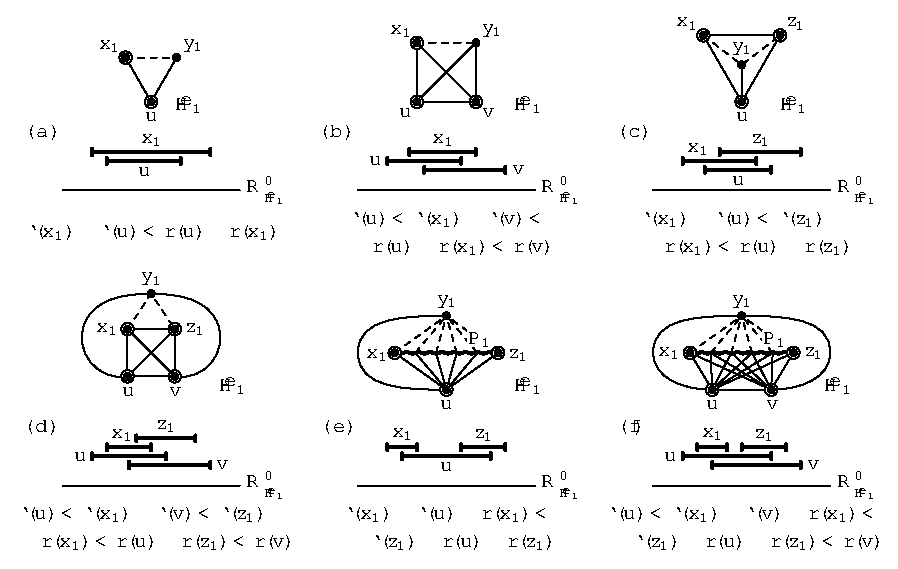
\includegraphics{definition_of_obstructions_BI_obstructions.eps}
\caption{All minimal 1-BI obstructions are depicted.  Each gives several $1$-BI obstructions with
different $\calR'_{\widetilde H_1}$, since there are several possible orderings of the endpoints
satisfying the given inequalities.  We have $x_1=z_1$ for (a) and (b), and $x_1 \ne z_1$ otherwise.
We have $u=v$ for (a), (c) and (e), and $u \ne v$ otherwise.}
\label{fig:BI_obstructions}
\end{figure}

\heading{$\boldsymbol{k}$-FS obstructions.} The class of \emph{forced side obstructions} is shown in
Fig.~\ref{fig:overview_of_obstructions}b.  To create $\widetilde H_k$ from $H_k$, we add a vertex
$u$ adjacent to $y_k$ and $z_k$. The partial representation contains three pre-drawn vertices $x_k$,
$y_k$ and $u$. We have $\ell(y_k) \le \ell(u) \le r(y_k) < r(u)$ and $\inter{x_k}'$ is on the
left of $\inter{y_k}'$. 

\heading{$\boldsymbol{k}$-EFS obstructions.}
The class of \emph{extended forced side obstructions} is similar to $k$-FS obstructions; see
Fig.~\ref{fig:overview_of_obstructions}c. To create $\widetilde H_k$ from $H_k$, we add $u$ adjacent
to $x_k$, $y_k$, and $z_k$, and $v$ adjacent to $y_k$ and $z_k$. The partial representation contains
four pre-drawn vertices $y_k$, $z_k$, $u$ and $v$ pre-drawn as follows:
$$\ell(u) < \ell(v) < \ell(y_k) \le r(y_k) < \ell(z_k) \le r(z_k) < r(u) \le r(v).$$

\heading{$\boldsymbol{k}$-FB obstructions.}
The class of \emph{forced betweenness obstructions} is similar to $k$-BI with $u=v$; see
Fig.~\ref{fig:overview_of_obstructions}d. To create $\widetilde H_k$ from $H_k$, we add $u$
adjacent to $y_k$ and $z_k$. The partial representation $\calR'_{\widetilde H_k}$ contains three
pre-drawn vertices $x_k$, $z_k$, and $u$.  We have $\ell(u) < \ell(z_k) \le r(u) \le r(z_k)$ and
$\inter{x_k}'$ is pre-drawn on the left of $\inter u'$.

\heading{$\boldsymbol{k}$-EFB obstructions.}
The class of \emph{extended forced betweenness obstructions} is similar to both $k$-BI and
$k$-FB; see Fig.~\ref{fig:overview_of_obstructions}e. To create $\widetilde H_k$ from $H_k$, we add $u$
adjacent to $x_k$, $y_k$ and $z_k$, and $v$ adjacent to $y_k$ and $z_k$. The partial representation
contains four pre-drawn vertices $x_k$, $z_k$, $u$, and $v$.  We have
$$\ell(u) < \ell(x_k) \le r(x_k) < \ell(v) < \ell(z_k) \le r(u) \le r(z_k) < r(v).$$

\heading{$\boldsymbol{k}$-FDS obstructions.}
The class of \emph{forced different sides obstructions} is shown in
Fig.~\ref{fig:overview_of_obstructions}f. To create $\widetilde H_k$ from $H_k$, we add $u$ adjacent
to $x_k$, $y_k$, and $z_k$, and $v$ adjacent to $y_k$ and $z_k$. The partial representation
contains three pre-drawn vertices $y_k$, $u$ and $v$ pre-drawn as follows:
$$\ell(u) < \ell(y_k) \le \ell(v) \le r(y_k) < r(u) \le r(v).$$

\heading{$\boldsymbol{k}$-EFDS obstructions.}
The class of \emph{extended forced different sides obstructions} is similar to $k$-FDS
obstructions; see Fig.~\ref{fig:overview_of_obstructions}g. To the construction of
$k$-FDS, we further add $w$ adjacent to $y_k$ and $z_k$.  The partial representation
contains four pre-drawn vertices $y_k$, $u$, $v$ and $w$ as follows:
$$\ell(u) < \ell(v) < \ell(y_k) \le \ell(w) \le r(y_k) < r(w) < r(u) \le r(v).$$

\heading{$\boldsymbol{k}$-FNS obstructions.} The class of \emph{forced nested side obstructions} is
constructed similarly as $k$-EFDS obstructions, but with $z_k$ pre-drawn instead of $y_k$; see
Fig.~\ref{fig:overview_of_obstructions}h. In $\calR'_{\widetilde H_k}$, we have
$$\ell(u) < \bigl\{\ell(v), \ell(w)\bigr\} \le \ell(z_k) \le r(w) < r(u) \le r(v),$$
where $\ell(v)$ and $\ell(w)$ are ordered arbitrarily.

\begin{figure}[t!]
\centering
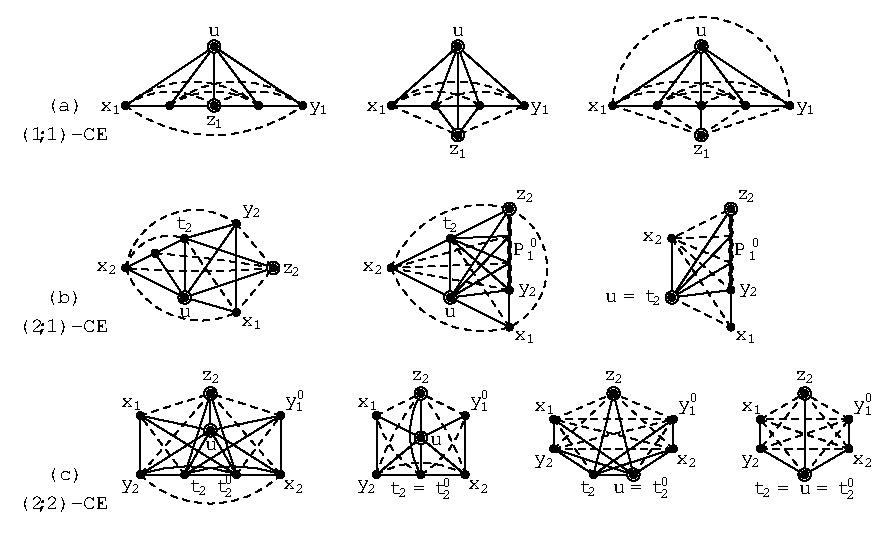
\includegraphics{definition_of_obstructions_kl_CE_obstructions.eps}
\caption[]{(a) There are three minimal $(1,1)$-CE obstructions, and they are all finite graphs. The
reason is that if, say, a path $P_1$ was very long, we could replace $x_1$ by an inner vertex of
$P_1$; so such an obstruction would not be minimal.\\
(b) There are three minimal $(2,1)$-CE obstructions. Due to the minimality, $P_2$ is a path of length at most
two.  When $x_2$ and $t_2$ are non-adjacent, then $P'_1 = y_2t_2z_2$ is a path
avoiding $N[x_2]$. When $x_2$ and $t_2$ are adjacent, there are two cases, namely, $u \ne t_2$, and
$u = t_2$.  The path $P'_1$ is of length at least two.\\
(c) There are four minimal $(2,2)$-CE obstructions, and they are all finite graphs. Necessarily
$x_2t_2$ and $y_2t'_2$ are edges, and we can choose $x_2$ in such a way that it is adjacent to
$y'_1$ (similarly, $y_2$ is adjacent to $x_1$). There are four different graphs, because the
vertices $u$, $t_2$ and $t'_2$ might be distinct or not.}
\label{fig:kl_CE_obstructions}
\end{figure}

\heading{$\boldsymbol{(k,\ell)}$-CE obstructions.}
The class of \emph{covered endpoint obstructions} is created from a $k$-FAT obstruction glued
to an $\ell$-FAT obstruction; see Fig.~\ref{fig:overview_of_obstructions}i.  To create
$\widetilde H_{k,\ell}$, we glue $H_k$ with $H'_\ell$.  We put $z_k = z'_\ell$, $x_k = y'_\ell$ and
$y_k = x'_\ell$, and some other vertices of these obstructions may be also shared.  We add $u$
adjacent to $x_k$, $y_k$, and $z_k$. The partial representation contains two pre-drawn intervals
$\inter{z_k}'$ and $\inter{u}'$ such that $\ell(u) < \ell(z_k) \le r(u) \le r(z_k)$. We always
assume that $k \ge \ell$.

In $(k,\ell)$-CE Lemma~\ref{lem:kl_ce}, we show that the only $(k,\ell)$-CE obstructions which are
minimal are $(k,1)$-CE obstructions and $(2,2)$-CE obstructions; so either $\ell = 1$, or $k = \ell
= 2$. For $k \ge 3$, a minimal $(k,1)$-CE obstruction consists of the subgraph $H_k$ of a $k$-FAT
obstruction together with a vertex $u$, where $u$ is either adjacent to all vertices of $H_k$, or $u
= t_k$.  The remaining $(k,\ell)$-CE obstructions, where $2 \ge k \ge \ell$, are depicted in
Fig.~\ref{fig:kl_CE_obstructions}.

\subsection{Proofs of Non-extendibility and Minimality}

We sketch proofs that the defined obstructions are non-extendible and minimal. This implies the
first part of Theorem~\ref{thm:repext_obstructions}.  We establish the harder implication in
Sections~\ref{sec:strategy}, \ref{sec:leaves}, \ref{sec:p_nodes}, \ref{sec:q_nodes}, and
\ref{sec:main_result}. 

\begin{lemma} \label{lem:correctness_k_FAT}
Every $k$-FAT obstruction is non-extendible and minimal.
\end{lemma}

\begin{proof}
We prove the claim by induction. For $k=1$, non-extendibility and minimality are clear. For
$k>1$, assume that $\inter{x_k}'$ is on the left of $\inter{y_k}'$, and $\inter{y_k}'$ is on the left of $\inter{z_k}'$. In every representation of
$k$-FAT, $\inter{t_k}$ covers $[\ell(y_k),\ell(z_k)]$.  We know that
$\inter{x_{k-1}}$ cannot be on the left of $\inter{x_k}'$, since $H_{k-1}$ is connected and $x_k$ is
non-adjacent to all vertices of $H_{k-1}$.  Therefore $\inter{x_{k-1}}$ has to be placed on the
right of $\inter{z_k}'$. We get a $(k-1)$-FAT obstruction, which is non-extendible by
the induction hypothesis.

It remains to argue the minimality. If one of $\inter{x_k}'$, $\inter{y_k}'$ and $\inter{z_k}'$ is
made free, we can place them in such a way that $\inter{z_k}$ is between $\inter{x_k}$ and
$\inter{y_k}$. This makes the partial representation extendible: It works for $k=1$, and for $k>1$,
we can place $x_{k-1}$ on the right of $\inter{y_k}$, which makes the induced $H_{k-1}$ extendible.
If we remove one of the vertices or induced paths, the argument is similar.\qed
\end{proof}

\begin{lemma} \label{lem:correctness_all}
The following obstructions are non-extendible and minimal:
\begin{packed_itemize}
\item SE, $k$-FS, $k$-EFS, $k$-FB, $k$-EFB, $k$-FDS, $k$-EFDS, and $k$-FNS obstructions,
\item $k$-BI obstructions for $k \le 2$,
\item $(k,\ell)$-CE obstructions where either $\ell = 1$, or $k=\ell=2$.
\end{packed_itemize}
\end{lemma}

\begin{proof}
For SE obstructions, the proof is trivial. For the remaining classes (aside $k$-BI and
$(k,\ell)$-CE), we proceed as follows. Non-extendibility follows from the fact that, in all cases,
$\inter{y_k}$ is forced to be placed between $\inter{x_k}$ and $\inter{z_k}$. To show minimality, we
use the minimality of $k$-FAT obstructions. Then it is easy to show that freeing any added pre-drawn
interval or removing any added vertex results in the possibility of placing $\inter{z_k}$ between
$\inter{x_k}$ and $\inter{y_k}$.

Consider a $k$-BI where $k \le 2$.  Non-extendibility follows from the fact that $\inter{y_k}$ has
to be placed between $\inter{x_k}'$ and $\inter{z_k}'$, thus forcing the k-FAT obstruction,
which is non-extendible by Lemma~\ref{lem:correctness_k_FAT}.  By removing a vertex or an induced
path of $H_k$, it becomes extendible as argued in Lemma~\ref{lem:correctness_k_FAT}. By freeing
$\inter{u}'$ or $\inter{z_k}'$, we can place $\inter{y_k}$ on the right of $\inter{z_k}'$ which
makes the partial representation extendible. By freeing $\inter{v}'$ or $\inter{x_k}'$, we can place $\inter{y_k}$ on the
left of $\inter{x_k}'$, which also makes it extendible because $k \le 2$ and $x_2$ is adjacent to
$t_2$.

For $(k,\ell)$-CE, either $\inter{y_k}$ is between $\inter{x_k}$ and $\inter{z_k}'$ (non-extendible
due to the $k$-FAT obstruction), or $\inter{y_\ell}$ is between $\inter{x_\ell}$ and
$\inter{z_\ell}'$ (non-extendible due to the $\ell$-FAT obstruction). Minimality is also easy:
Removing or freeing $u$ allows to place $\inter{z_k}'$ between $\inter{x_k}$ and $\inter{y_k}$,
which is extendible. And removing anything from one of the FAT obstructions allows one of the
orderings of $\inter{x_k}$ and $\inter{y_k}$ to be extendible.\qed
\end{proof}

We note that the list of minimal obstructions is unique. Indeed, every minimal obstruction itself
corresponds to a valid input, which cannot be obstructed by a distinct obstruction due to the
minimality. Therefore, it is not possible to construct a smaller list of minimal obstructions, or to
argue that if the partial representation contains a particular obstruction, then it also contains an
additional one.
